\section{\pwTwo}

\begin{figure*}[ht]
	\centering
	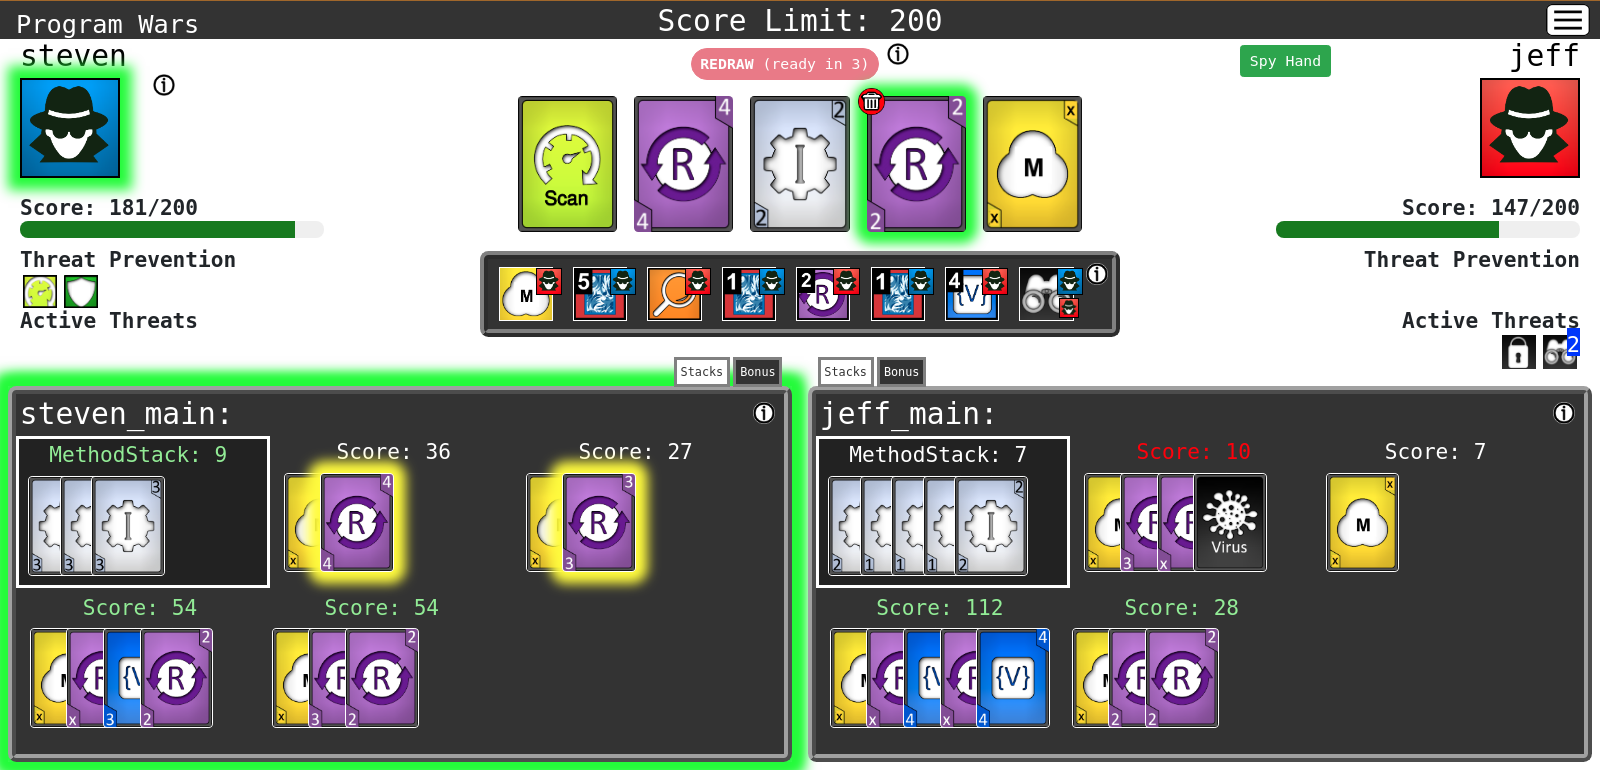
\includegraphics[width=\textwidth]{images/game.PNG}
	\caption{Partway through a game.}
	\label{fig:game}
\end{figure*}

This section presents a high-level view of the gameplay and a detailed description of the cards that teach programming fundamentals and cybersecurity in \pwTwoNS. 

\subsection{Gameplay Overview}
At the start of the game, a player can choose to play either against another human on the same computer (i.e. hot-seat play) or against provided computer opponents. \pwTwo expands the original game with two modes of gameplay: \emph{Beginner} and \emph{Standard}. For each gameplay mode, the player can choose to play with one of four different sets of cyberattack and cyberdefense cards, adding them to the game's basic deck.\footnote{A basic \gameName deck is comprised of only \Ins, \Mns, \Rns, \Vns, \Serns, \Sort and \Scan cards.}

In \B mode, only one of the two types of cyberattack cards are added to the deck - either two malware cards or two hack cards. In \Std mode, the player can choose to play with either all of the malware cards, all of the hack cards, or two different combinations of two malware and two hack cards. Each card set includes the corresponding cybersecurity cards that block the added attacks. These card sets change the gameplay difficulty through the different combinations of cybersecurity and cyberattack cards. The game uses these cards sets to progressively introduce more complicated cards. Table \ref{table:cardSets} shows the different card sets in each gameplay mode. 

\begin{table*}
	\caption{Game modes and Card sets in \pwTwoNS.}
	\begin{tabular}{|c|c|c|c|c|c|c|c|c|c|}
		\cline{1-10}
		& & \multicolumn{4}{|c|}{Beginner} & \multicolumn{4}{|c|}{Standard} \\ 
		\cline{3-10}
		Type & Card & Malware 1 & Hack 1 & Malware 2 & Hack 2 & Malware & Hack  & Combined 1 & Combined 2 \\ \hline
		\hline
		\multirow{2}{*}{Safety} & AntiVirus 	& X & & X & & X & & X & X \\ \cline{2-10}
		& Firewall 	&  & X &  & X &  & X & X & X \\ \hline \hline
		\multirow{4}{*}{Malware} & Spyware 	& X & & & & X & & X & \\ \cline{2-10}
		& Ransomware 	& X & & & & X & &  & X \\ \cline{2-10}
		& Virus		& & & X & & X & & X &  \\ \cline{2-10}
		& Trojan 		& & & X & & X & &  & X  \\ 
		\hline
		\hline
		\multirow{4}{*}{Hack} & Buffer Overflow 	& & X & & & & X & X & X \\ \cline{2-10}
		& Cross-site Scripting 	& & & & X & & X & & \\ \cline{2-10}
		& DoS Attack		& & X & & & & X & & X \\ \cline{2-10}
		& SQL Injection	& & & & X & & X & X &  \\ 
		\hline 
	\end{tabular}
	\label{table:cardSets}
\end{table*}

At the start of a game, each player is dealt five cards and the player receives another card from the deck at the end of each turn. \gameName is played in a series of rounds in which each player takes a turn to either play or discard a card from their hand, or discard and draw a new hand. A player needs to create a program that reaches the goal number of points to win the game. The points represent the total number of instructions that would be executed by the computer-based on the cards in play. Players use a variety of cards to build their program, while also fending off attacks from their opponents.

If either player has reached or exceeded the goal number of points, the game will finish at the end of the current round. This makes it possible for both players to reach the goal number of points in a game. In \B mode, the player's instruction score is all that is used to determine the winner, and players can tie. In \Std mode, bonus points are awarded for reaching specific objectives, such as the use of \R and \V cards, or ending the game without being under the influence of cyberattacks. If both players have the same total score, these bonus points are used to break ties (i.e. the player who used the most \V cards wins). If this method cannot determine a winner, the players tie.

\subsection{Gameplay Areas}

Figure \ref{fig:game} shows part of the way through a two-player game. The top right and top left corners of the screen show the status of each player. The player's name is shown along with a unique image that is highlighted with green on their turn. In Figure \ref{fig:game} it is currently Steven's turn. Under each player's image are their score and a progress bar showing their progress towards the goal number of points.\footnote{The bar is red if the player is below 50\% of the goal number of points, yellow if below 75\%, and green above 75\%.} Below the player's score is an area to show their current status effects. Status effects are represented by small icons, usually a smaller version of the image from the card that caused the effect. The \emph{Threat Prevention} section shows the current cybersecurity effects active for the player. In Figure \ref{fig:game}, Steven has a \Scan and \Anti effect active. The \emph{Active Threats} section shows any cyberattacks affecting the player. Figure \ref{fig:game} shows that Jeff has been attacked by \Ran and \Spyns. Effects that last for a specific number of turns are shown with the number of turns remaining over the top right corner. In the example game, the \Spyns 's effect on Jeff has only two turns until it expires. The status effects are added and removed as cyberattack and cybersecurity cards are played. Further details about cybersecurity and cyberattack cards and their effects are provided in Sections \ref{section:malware} and \ref{section:hacking}.

Each of the gameplay play areas contains an \emph{Information} icon (an $i$ within a circle) that when clicked on provides a short description of that play area.

\subsubsection{\Hand:}
The top of the centre area of Figure \ref{fig:game} shows the current player's hand with the player's currently selected card highlighted with green. When a card is selected, a small trash can icon appears in the upper lefthand corner of the card to allow the player to discard it. Above the cards is a button to allow the player to redraw their hand. If a player redraws their hand, they must wait for three (3) turns to do so again. In Figure \ref{fig:game}, the \emph{Redraw} button is inactive and shows that there are three turns until Steven (the current player) can use it again. 

Most cards are played by dragging the card from the hand and dropping the card where it is to be added - either the \Play or \MS areas of the \Prg. Algorithm, cybersecurity, and cyberattack cards (excluding \Vins) are played by clicking on them. When these cards are selected, a small overlay appears over the card allowing the player to make a choice. For algorithm cards, the overlay has a single button to activate the card. Safety cards have the same \texttt{Activate} button when the card can be activated. However, if the same effect is already applied to the player, then the overlay will indicate that the effect is already active, and the card will not be playable. For cyberattack cards, the overlay will give a set of buttons for valid targets of the attack. The overlay will display ``No Targets" if there are no valid targets for the attack. Some cyberattack effects will not allow certain cards to be played. Cards that cannot be played will be highlighted red while in the player's hand and will not be draggable or show an overlay when selected.

\subsubsection{\Hist:}
Below the player's hand is a visual representation of the last eight turns played. Each icon represents a card that was played. In the top right corner of each of these icons is the image of the player that played that particular card. In Figure \ref{fig:game}, the leftmost icon shows that Jeff played a \M card last turn. If a card had a target player, the target's image is placed on the bottom right corner of the card icon. This can be seen on the rightmost icon in the turn history in Figure \ref{fig:game} where it shows that Steven played a \Spy card on Jeff. Some cards may include another card or effect, such as \Scan when it removes an effect. In this case, a small icon for the card or effect included will be placed on the bottom left corner of the card image (not shown). As the game progresses, the leftmost icon is replaced by the latest card played and all icons are shifted one position to the right.

\subsubsection{\Prg:}
The bottom half of the screen represents an editor where the player builds their program. Programs are built by creating stacks of \Ins, \Mns, \R and \V cards. Each stack of cards represents a portion of the player's program. An \I or \M card can be dragged and dropped onto the \Prg~ to start a new stack. \R \\
and \V cards are played by dropping them onto an existing stack. A stack with a highlight around the top card indicates that the currently selected card can be played on that stack. If the valid stack is in the current player's \Prg, the highlight will be yellow. For cyberattack cards, such as \Vins, the valid stack will be in an opponent's \Prg and the highlight will be red. In Figure \ref{fig:game}, the currently selected \R card from Steven's hand can be played on one of the two highlighted stacks.

Each stack shows its score above it telling the player how many points that stack is contributing to the player's score. The \MS area, which is surrounded by a white border, is a special stack that only accepts instruction cards. The \MS score is the score used for the \M card, is capped at nine (9) points and the stack can hold a maximum of six (6) \I cards. Placing too many low value \I cards in a \MS can leave a player unable to reach the stack's maximum score.

The total score for a player is the sum of all of their stack scores, excluding the \MSns. Stacks with green scores indicate that the stack is complete\footnote{A stack is considered complete when it has two (2) \R cards played on it. \Rx cards only count towards completing a stack if they are paired with a \V card.} and no more cards can be added to it. A stack with a red score indicates that the stack is not contributing its full value to the total score. For example, the stack in Jeff's play area with the \Vi card on top should contribute 21 points (7 for the \M card times 3 for the \Rns-3). However, the \Vi card reduces the stack's value by half to 10 (see Section \ref{section:malware} for details). 

\subsubsection{\Goals:}
In \Std mode, a player can achieve bonus points by reaching certain goals during a game. A player's current bonus points can be seen by switching their play area to the \Bns tab. The tabs are in the centre of the screen attached to the \Prg~ of each player. This tab is not shown for a computer opponent to prevent human players from seeing a computer opponent's bonus progress. The \Bns area, shown in Figure \ref{fig:bonus}, has a set of conditional statements written in a C-like pseudocode and replaces the \texttt{True} and \texttt{False} playfields in \pwOne.

The conditional portion of the statement identifies for what the bonus is awarded. Some bonuses are for playing cards (i.e. \texttt{True} when playing a \R card), and others are for maintaining a certain status (i.e. not being affected by cyberattacks). The body of the condition shows the number of points a player will receive for satisfying the condition. If the text is red, it means the condition is not met, and the text will turn green when the player satisfies the condition. Some conditions, such as the \texttt{(no\_malware \&\& no\_hacks)} condition, may be gained or lost during the game.

At the end of each turn, the player's bonuses are re-calculated and the total bonus score is updated and shown at the top of the \Bns tab. Bonus scores are only added to the player's instruction score once the game has finished and do not apply towards reaching the goal score during the game. These bonuses are intended to help reinforce certain concepts and motivate the player towards what can be considered as good programming practices.

\begin{figure}[ht]
	\centering
	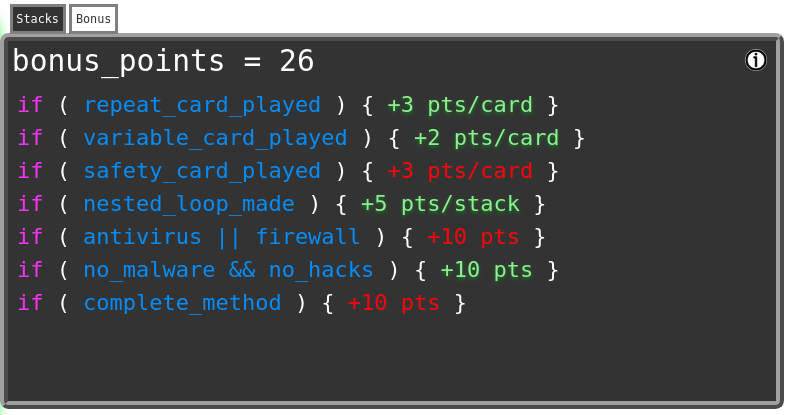
\includegraphics[width=\columnwidth]{images/objectives.PNG}
	\caption{The \Bns tab for a player.}
	\label{fig:bonus}
\end{figure}
